\section{Formalization}
\label{sec:formalization}

In this section, we formalize the Atomic Swap protocol \MOD{(the original version on Bitcointalk~\cite{nolan2013alt})} and the American Call Option,
then prove that the Atomic Swap is equivalent to an American Call Option without the premium.



\begin{figure}
    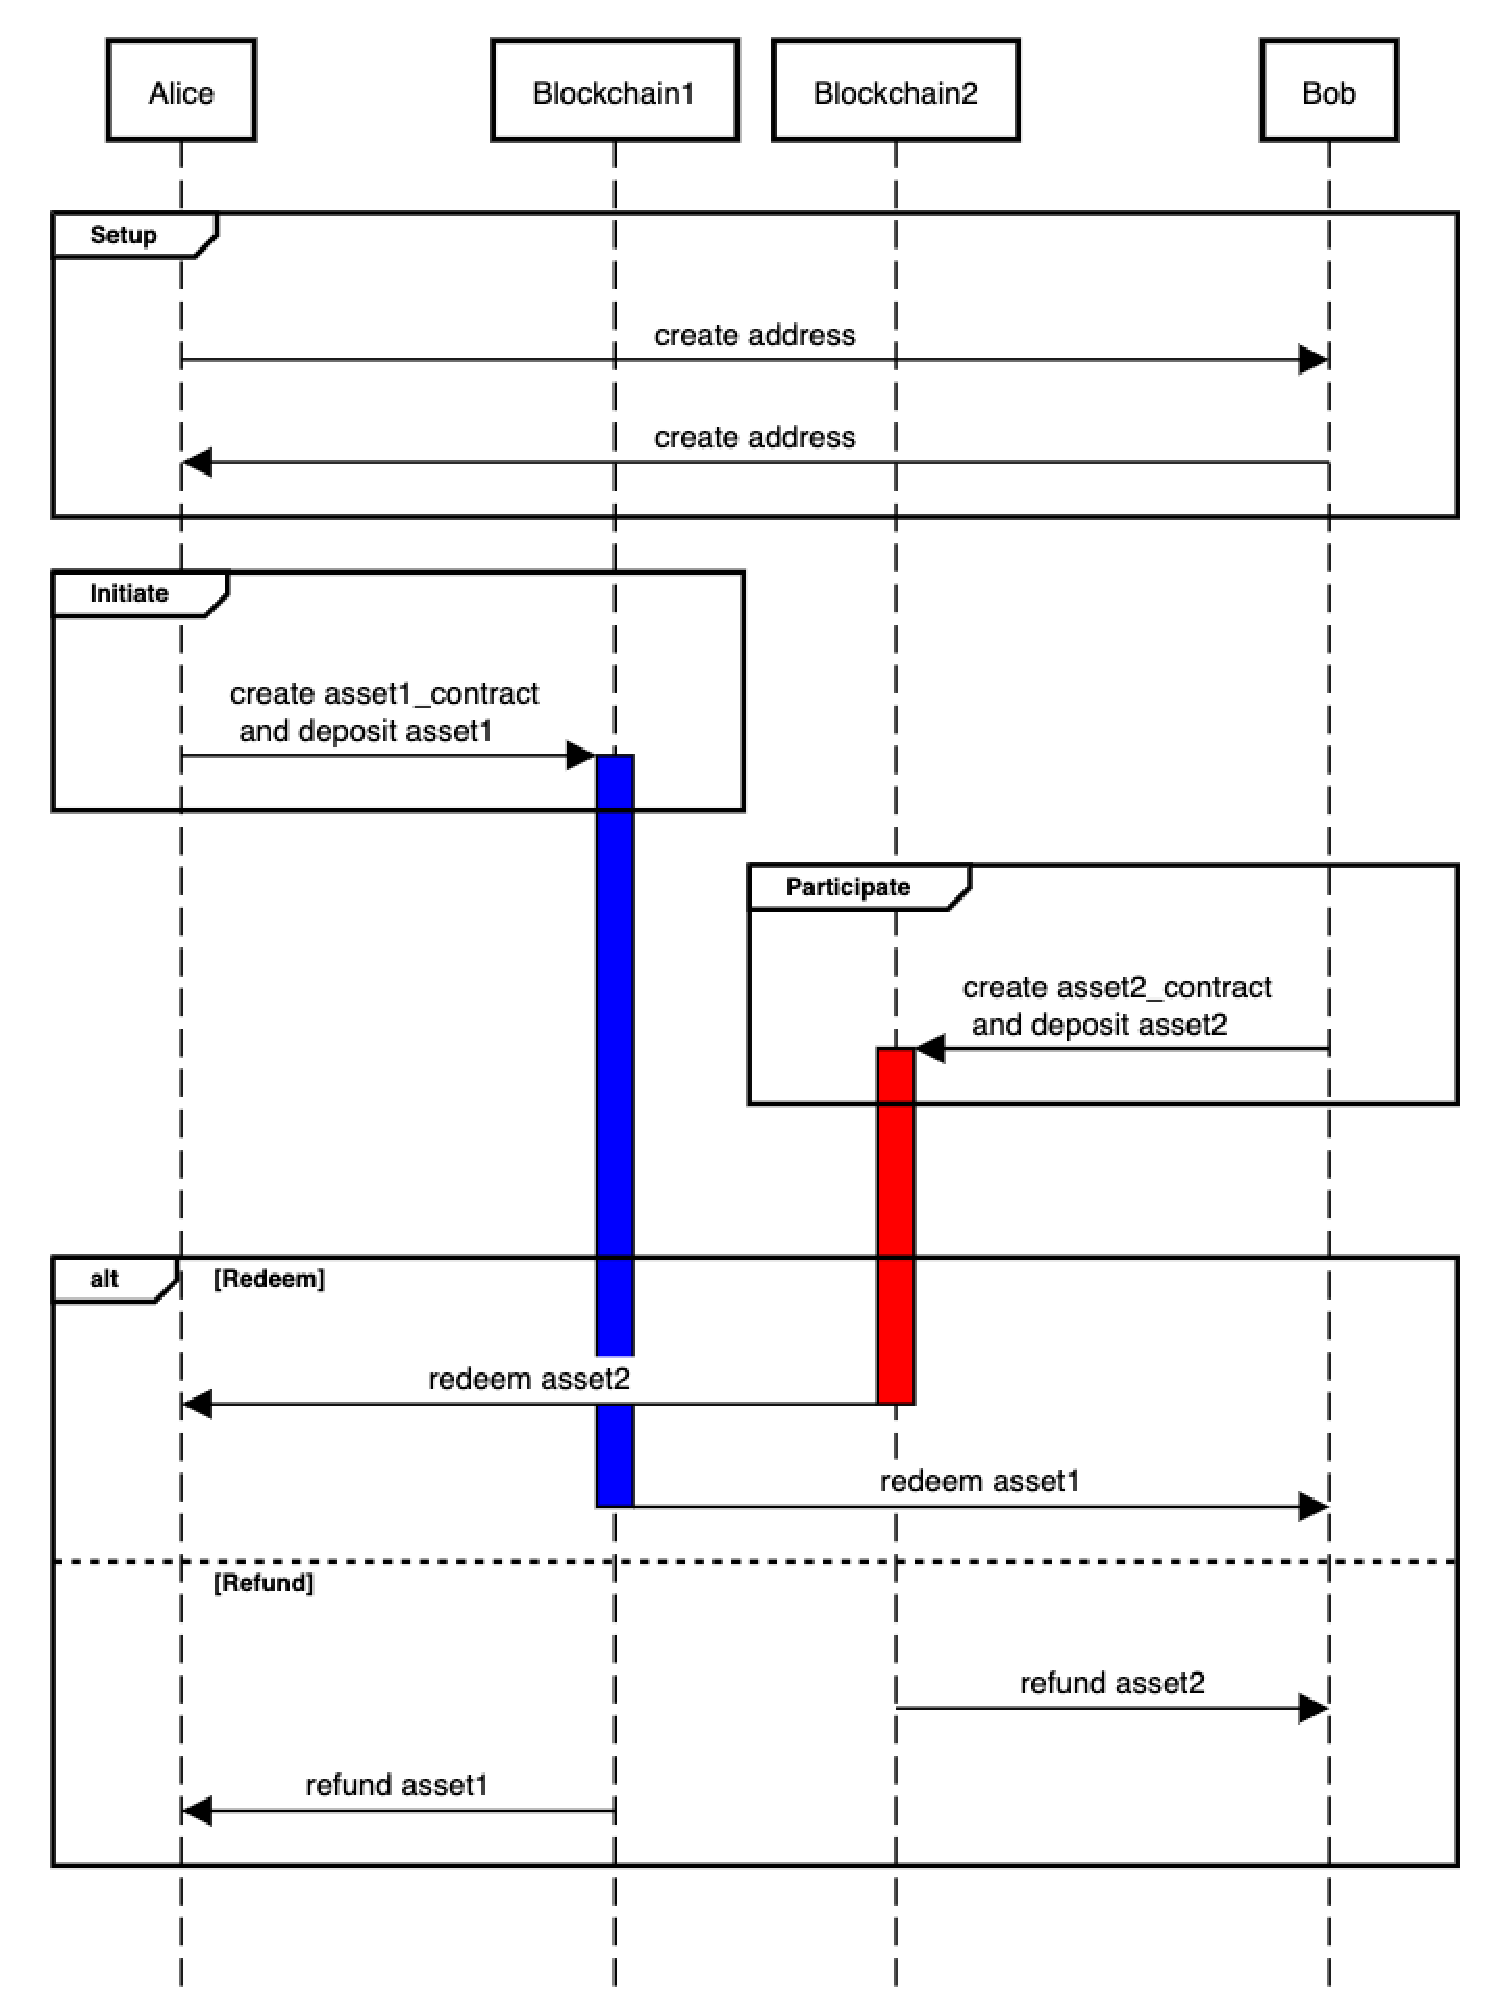
\includegraphics[width=.7\linewidth]{sequence_diagram_original.eps}
    \caption{Sequence diagram of the Atomic Swap.}
    \label{fig:sequence_diagram_original}
\end{figure}

\begin{figure}
    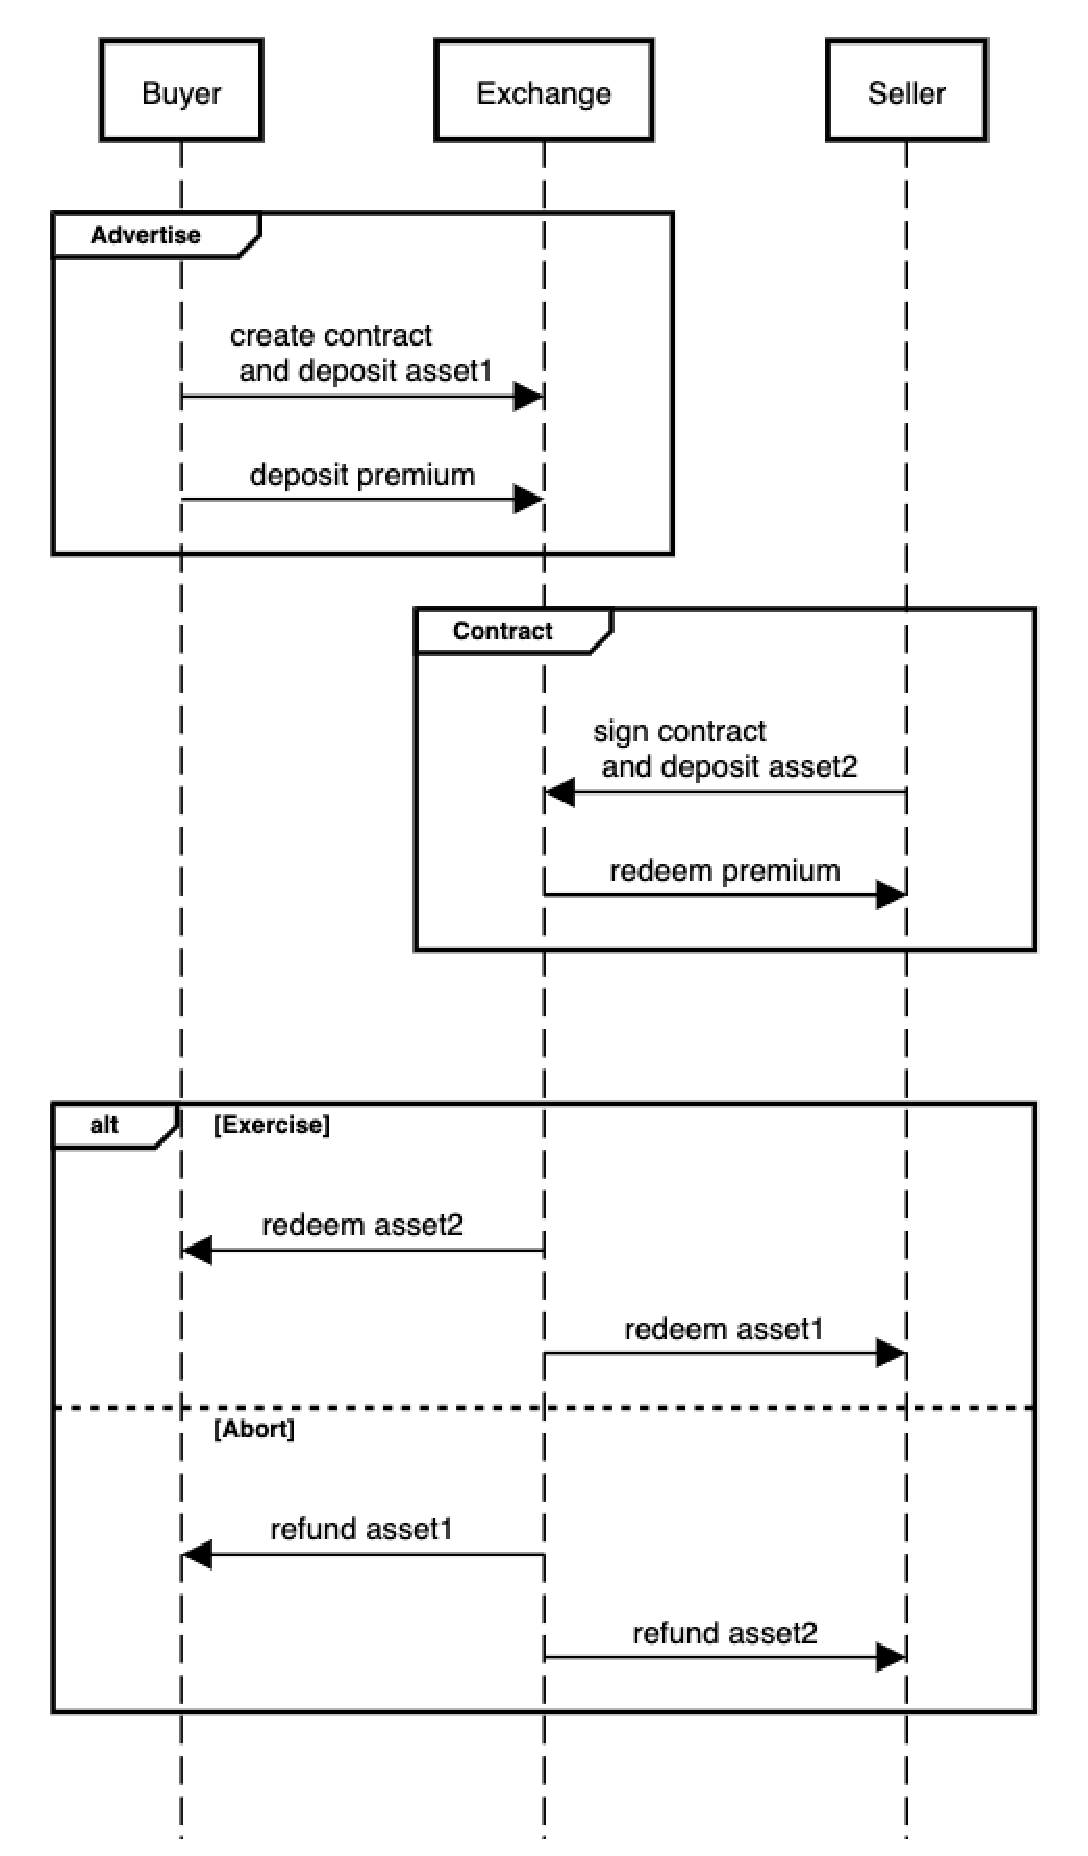
\includegraphics[width=.7\linewidth]{sequence_diagram_option.eps}
    \caption{Sequence diagram of the American Call Option.}
    \label{fig:sequence_diagram_option}
\end{figure}





\subsection{Atomic Swap}

\MOD{We formalise the original version of the Atomic Swap~\cite{nolan2013alt}.

\subsubsection{Security assumptions}

Before the formalization, we give security assumptions on the Atomic Swap.

First, we assume blockchains involved in the Atomic Swap are secure, and execute all transactions correctly.
The Atomic Swap is based on blockchains.
If the blockchains are insecure, the Atomic Swap will also be insecure.

Second, we assume the HTLC mechanism in blockchains is reliable.
More specifically,
1) blockchains produce new blocks with stable speeds;
2) the hash algorithm used by HTLCs is secure;
3) the runtime for executing HTLCs is reliable.


Third, the time for confirming a transaction is negligible compared to timelocks.
In practice, the swap initiator's timelock is 48 hours and the swap participant's timelock is 24 hours by default~\cite{nolan2013alt}, while confirming a transaction is less than 1 hour for most blockchains.

}

\subsubsection{Process}

We denote the initiator in the Atomic Swap as Alice, and the participant as Bob.

\begin{definition}
We define an Atomic Swap $\mathcal{AS}$ as

$$\mathcal{AS} = (x_1, Coin_1, x_2, Coin_2)$$

where Alice hopes to buy $x_2$ $Coin_2$ on blockchain $BC_2$ from Bob with $x_1$ $Coin_1$ on blockchain $BC_1$.
\end{definition}

The Atomic Swap protocol consists of five algorithms:
\textbf{Setup},
\textbf{Initiate},
\textbf{Participate},
\textbf{Redeem}, and
\textbf{Refund}.

\paragraph{\textbf{Setup}($\lambda, id, BC_i$)}
\textbf{Setup}($\cdot$) takes a security parameter $\lambda$,
the invoker identify $id \in \{A, B\}$,
and the blockchain identities $BC_i$ where $i \in \{1, 2\}$.
It returns the secret key $sk_{id, i}$, the public key $pk_{id, i}$ and the address $\beta_{id, i}$ on the blockchain $BC_i$ for the invoker $id$.
Note that with $sk_{id, i}$, anyone can produce $pk_{id, i}$, and with $pk_{id, i}$ anyone can produce $\beta_{id, i}$. But these cannot be done in the inverse manner.

\paragraph{\textbf{Initiate}($x_1, sk_{A, 1}, \beta_{B, 1}, s, \delta_1$)}
\textbf{Initiate}($\cdot$) can only be invoked by Alice, which is guaranteed by the ownership of $sk_{A, 1}$.
% input
It takes the amount $x_1$ of Alice's $Coin_1$,
Alice's secret key $sk_{A, 1}$ on $BC_1$,
Bob's address $\beta_{B, 1}$ on $BC_1$,
the random secret $s$ chosen by Alice,
and the timelock $\delta_1$ (which is a timestamp) picked by Alice.
% output
It returns the secret hash $h$,
the contract script $\mathcal{C}_1$,
the contract transaction $tx_{\mathcal{C}, 1}$,
the refund script $\mathcal{R}_1$,
and the refund transaction $tx_{\mathcal{R}, 1}$.
% description s/h
The preimage $s$ is a random string generated by Alice. At this stage, $s$ is only known to Alice.
The preimage hash $h = \mathcal{H}(s)$, where $\mathcal{H}$ is a secure hash function.
$h$ is published when triggering \textbf{Initiate}($\cdot$).
% description contract, tx
The contract script $\mathcal{C}_1$ is that ``Alice pays $x_1$ $Coin_1$ from $\beta_{A, 1}$ to $\beta_{B, 1}$ if Bob can provide $s$ before or on a timelock $\delta_1$. After $\delta_1$, Alice can refund the money - get $x_1$ $Coin_1$ back.''
$\mathcal{C}_1$ will be published as a transaction $tx_{\mathcal{C}, 1}$ on $BC_1$ when triggering \textbf{Initiate}($\cdot$).
The refund script $\mathcal{R}_1$ is that ``Alice pays $x_1$ $Coin_1$ from $\beta_{A, 1}$ to her another address.'' This is to ensure $x_1$ $Coin_1$ can no longer be redeemed by others. Alice can do this only after $\delta_1$.
% The refund is done by publishing $\mathcal{R}_1$ as a transaction $tx_{\mathcal{R}, 1}$ on $BC_1$ if Alice can and decide to refund.

\paragraph{\textbf{Participate}($x_2, sk_{B, 2}, \beta_{A, 2}, h, \delta_2$)}
\textbf{Participate}($\cdot$) can only be invoked by Bob, which is guaranteed by the ownership of $sk_{B, 2}$.
% input
It takes the amount $x_2$ of Bob's $Coin_2$,
Bob's secret key $sk_{B, 2}$ on $BC_2$,
Alice's address $\beta_{A, 2}$ on $BC_2$,
the amount $x_2$ of Bob's $Coin_2$
and the secret hash $h$.
% output
It returns the contract script $\mathcal{C}_2$,
the contract transaction $tx_{\mathcal{C}, 2}$,
the refund script $\mathcal{R}_2$,
and the refund transaction $tx_{\mathcal{R}, 2}$.
% description contract, tx
The contract script $\mathcal{C}_2$ is that ``Bob pays $x_2$ $Coin_2$ from $\beta_{B, 2}$ to $\beta_{A, 2}$ if Alice can provide $s$ before or on a timelock $\delta_2$ (which is a timestamp). After the time of $\delta_2$, Bob can refund the money - get $x_2$ $Coin_2$ back.''
Here $\delta_2$ should expire earlier than $\delta_1$.
The contract script is published as a transaction $tx_{\mathcal{C}, 2}$ on $BC_2$ when triggering \textbf{Initiate}($\cdot$).
The refund script $\mathcal{R}_2$ is that ``Bob pays $x_2$ $Coin_2$ from $\beta_{B, 2}$ to his another address.'' This is to ensure $x_2$ $Coin_2$ can no longer be redeemed by others. Bob can do this only after $\delta_2$.
% The refund is done by publishing $\mathcal{R}_2$ as a transaction $tx_{\mathcal{R}, 2}$ on $BC_2$ if Bob can and decide to refund.

\paragraph{\textbf{Redeem}($sk_{id, i}, s, tx_{\mathcal{C}, i}$)}
\textbf{Redeem}($\cdot$) can be invoked by both parties, but with the condition $(id = A \wedge i = 2) \vee (id = B \wedge i = 1)$.
% input
It takes the secret key $sk_{id, i}$,
Alice's random secret $s$,
and the payment transaction $tx_{\mathcal{C}, i}$.
% output
It returns $\mathcal{V} \in \{0, 1\}$ indicating if the redemption is successful or not.
In the beginning, \textbf{Redeem}($\cdot$) will check if $\delta_i$ has expired or not. If $\delta_i$ has expired, \textbf{Redeem}($\cdot$) returns $0$ directly, otherwise it will proceed.
Either Alice or Bob can perform the redemption if knowing $s$, but recall that only Alice knows $s$ at the beginning.
As Alice knows $s$, she can redeem $x_2$ $Coin_2$ in $tx_{\mathcal{C}, 2}$ to her account $\beta_{A, 2}$ by providing $s$.
After Alice triggers \textbf{Redeem}($\cdot$), $s$ is published and revealed to everyone including Bob, so that Bob can redeem $x_1$ $Coin_1$ to his account $\beta_{B, 1}$ in $tx_{\mathcal{C}, 1}$ by providing $s$ as well.

\paragraph{\textbf{Refund}($sk_{id, i}, tx_{\mathcal{R}, i}$)}
\textbf{Refund}($\cdot$) can be invoked by both parties, but with the condition $(id = A \wedge i = 1) \vee (id = B \wedge i = 2)$.
It takes the secret key $sk_{id, i}$,
and the refund transaction $tx_{\mathcal{R}, i}$.
It returns the $\mathcal{V} \in \{0, 1\}$ indicating if the refund is successful or not.
In the beginning, \textbf{Refund}($\cdot$) will check if $\delta_i$ has expired or not. If $\delta_i$ is still valid, \textbf{Refund}($\cdot$) returns $0$ directly, otherwise it will proceed.
Both Alice and Bob can perform the refund by publishing $tx_{\mathcal{R}, i}$ after the timelock $\delta_i$, respectively.

% procedure
\paragraph{Process.}
Figure~\ref{fig:sequence_diagram_original} shows the Atomic Swap process.
More specifically, Alice and Bob proceeds the Atomic Swap as follows:
Alice and Bob first creates secret keys, public keys and addresses by triggering \textbf{Setup}($\cdot$), then they exchange those generated addresses.
Alice then triggers \textbf{Initiate}($\cdot$) to initiate the swap $\mathcal{AS}$, and Bob triggers \textbf{Participate}($\cdot$) to participate in $\mathcal{AS}$.
Within $\delta_2$ Alice can redeem $x_2$ $Coin_2$ by triggering \textbf{Redeem}($\cdot$), then Bob can redeem $x_1$ $Coin_1$ by triggering \textbf{Redeem}($\cdot$).
In this case, $\mathcal{AS}$ succeeds for both Alice and Bob.
However, Alice can also keep not triggering \textbf{Redeem}($\cdot$) and wait for $\delta_2$ to expire.
After $\delta_2$ expires, Bob can refund $x_2$ $Coin_2$ by triggering \textbf{Refund}($\cdot$), and Alice can refund $x_1$ $Coin_1$ by triggering \textbf{Refund}($\cdot$) after $\delta_1$ expires.
In this case, $\mathcal{AS}$ fails for both Alice and Bob.

% why atomic
We can see that $\mathcal{AS}$ either succeeds or fails for both Alice and Bob.
In detail,

\begin{itemize}
    \item If Alice misbehaves when triggering \textbf{Setup}($\cdot$) or \textbf{Initiate}($\cdot$), Bob will lose nothing as he hasn't deposited $Coin_2$ yet.
    \item If Bob misbehaves when triggering \textbf{Participate}($\cdot$), Alice can choose to abort $\mathcal{AS}$ by triggering \textbf{Refund}($\cdot$).
    \item Alice can only choose to \textbf{Redeem}($\cdot$) $Coin_2$ or wait $\delta_2$ to expire.
    Once Alice triggers \textbf{Redeem}($\cdot$), Bob can also trigger \textbf{Redeem}($\cdot$).
    Once $\delta_2$ expires, Bob can trigger \textbf{Refund}($\cdot$) to get his $x_2$ $Coin_2$ back.
\end{itemize}

% misuse
However, one may take both $Coin_1$ and $Coin_2$ if the other does not trigger \textbf{Redeem}($\cdot$) or \textbf{Refund}($\cdot$) on time.
For example, if Bob does not trigger \textbf{Redeem}($\cdot$) after Alice triggers \textbf{Redeem}($\cdot$) and $\delta_1$ expires, Alice can also refund $x_1$ $Coin_1$ by triggering \textbf{Refund}($\cdot$).
But in this case it is Bob to blame, because he should have had enough time - at least $\delta_2 - \delta_1$ \MOD{(48 - 24 = 24 hours by default)} - to redeem $x_1$ $Coin_1$.
Another example is that Alice broadcasts the transaction of \textbf{Redeem}($\cdot$) after $\delta_2$, but Bob has already triggered \textbf{Refund}($\cdot$).
Therefore, Bob can also trigger \textbf{Redeem}($\cdot$) with the preimage in Alice's transaction of \textbf{Redeem}($\cdot$) before $\delta_1$.
Similarly, it is Alice to blame, because she should have had enough time - before $\delta_2$ - to trigger \textbf{Redeem}($\cdot$).

% def S_t
Similar to conventional finance assets, $Coin_2$'s value is also fluctuating due to the market mechanism.
We denote the asset's underlying value (with the unit $\frac{Coin_2}{Coin_1}$) at the time $t$ as $S_t$.















\subsection{American Call Option}

The American Call Option is a contract that ``one can buy an amount of an asset with an agreed price prior to or on an agreed time in the future''. 
The agreed price is usually called the \textit{spot price}, and the buying is called \textit{exercising}.
For American Call Option, the option buyer can exercise in advanced of the agreed exercise time.
The price of the asset when exercising is called the \textit{strike price}.
As mentioned in Section~\ref{subsec:background_option}, the option contract itself has value, and its value is called the \textit{premium}.
The option buyer should pay for both the asset and the premium when participating in the contract.

Formally,

\begin{definition}
We define an American Call Option contract $\Pi$ as

$$\Pi = (\pi_1, \pi_2, K, A, T, C)$$

where
$\pi_1$ and $\pi_2$ are the currency of the option buyer and the asset of the option seller, respectively; 
$K$ is the strike price with the unit $\pi_2 / \pi_1$ \HY{isnt it  $\pi_1 / \pi_2$?}- the price of $\pi_2$ measured in $\pi_1$;
$A$ is the amount of the asset $\pi_2$ that the option seller wants to sell;
$T$ is the agreed strike time;
$C$ is the \textit{premium} with the unit $\pi_1$.
\end{definition}

The process of an American Call Option is as follows:

\begin{enumerate}
    \item \textbf{Advertise}: The option seller creates and advertises an American Call Option contract $\Pi = (\pi_1, \pi_2, K, A, T, C)$.
    \item \textbf{Contract}: The option buyer finds $\Pi$ is profitable, so he participates in $\Pi$.
    To participate, the option buyer should pay $C$ to the option seller first.
    Note that the option buyer does not pay for $A$ $\pi_2$ at this stage.
    Also note that the option seller cannot abort $\Pi$ after the option buyer participates in $\Pi$.
    \item \textbf{Exercise} or \textbf{Abort}: The option buyer exercises $\Pi$ - pays $AK$ $\pi_1$ to the option seller - before or on $T$, and the option seller gives $A$ $\pi_2$ to the option buyer.
    If the option buyer does not exercise $\Pi$ before or on $T$, $\Pi$ will abort - the option buyer gets $\pi_1$ back and the option seller gets $\pi_2$ back and $C$. In other words, both of them get their underlying asset back, but the option buyer loses the premium $C$.
\end{enumerate}

% asset underlying value
The underlying value of $\pi_2$ is fluctuating over time due to the market mechanism.
Intuitively, if the price of $\pi_2$ rises when the option buyer exercises $\Pi$, the option buyer profits, because he buys $\pi_2$ with the price lower than the current market price.
Formally, we denote the asset's underlying value (with the unit $\pi_2 / \pi_1$) at the time $t$ as $S_t$.
Assume the option buyer exercises $\Pi$ at a time $T' \leq T$, he can profit $[(S_{T'} - K) A - C]$ $\pi_1$.













\subsection{An Atomic Swap is a premium-free American Call Option}

We show that an Atomic Swap is equivalent to a premium-free American Call Option.

More specifically,

\begin{theorem}
$\mathcal{AS} = (x_1, Coin_1, x_2, Coin_2)$ is equivalent to the American Call Option contract

$$
\Pi = (Coin_1, Coin_2, \frac{x_2}{x_1}, x_2, \delta_2, 0)
$$

where:
\textbf{Advertise} in the American Call Option is equivalent to \textbf{Setup}($\cdot$) and \textbf{Initiate}($\cdot$) in the Atomic Swap;
\textbf{Contract} in the American Call Option is equivalent to \textbf{Participate}($\cdot$) in the Atomic Swap;
\textbf{Exercise} in the American Call Option is equivalent to \textbf{Redeem}($\cdot$) in the Atomic Swap;
\textbf{Abort} in the American Call Option is equivalent to \textbf{Refund}($\cdot$) in the Atomic Swap.

\end{theorem}


\begin{proof}

In the American Call Option context, the option buyer Alice wants to buy $x_2$ $Coin_2$ from the participant Bob by using $x_1$ $Coin_1$.
$Coin_1$ is the currency Alice uses, $Coin_2$ is the asset Bob has.
$\frac{x_2}{x_1}$ is the price of the asset from Alice's perspective, so $\frac{x_2}{x_1}$.
$\delta_2$ is the timelock of the contract transaction on $BC_2$.
It is equivalent to the strike time of $\Pi$, because after $\delta_2$ Bob can refund his asset back and invalidate $\mathcal{AS}$, but before $\delta_2$ Bob cannot abort $\mathcal{AS}$ if Alice \textbf{Participate}s.
Establishing the Atomic Swap does not require Alice to pay anything other than the asset to Bob, so the premium here is zero.
\end{proof}